\documentclass[journal]{IEEEtran}
\usepackage{blindtext}
\let\labelindent\relax
\usepackage[inline]{enumitem}
\usepackage{graphicx}
\usepackage[acronym,toc,shortcuts]{glossaries}
\usepackage{subcaption}
\usepackage[bookmarksopen, bookmarksdepth=2, breaklinks=true]{hyperref}
\usepackage[official]{eurosym}
\usepackage{listings}

% *** GRAPHICS RELATED PACKAGES ***
%
\ifCLASSINFOpdf
\else
\fi


\newacronym{mbaas}{MBaaS}{Mobile Backend as a Service}
\newacronym{sdk}{SDK}{Software Development Kit}
\newacronym{aws}{AWS}{Amazon Web Services}
\newacronym{api}{API}{Application Programming Interface}
\newacronym{rest}{REST}{Representational State Transfer}
\newacronym{iot}{IoT}{Internet of Things}
\newacronym{cdn}{CDN}{Content Delivery Network}
\newacronym{ide}{IDE}{Integrated Development Environment}

\hyphenation{op-tical net-works semi-conduc-tor}


\begin{document}
\title{Untersuchung der AWS Mobile Hub}

\author{\begin{center}
 Michael Zipperle \\ 
 \textit{259564} \\
 Hochschule Furtwangen \\
 Michael.Zipperle@hs-furtwangen.de \\
\end{center}}%
        
% The paper headers
\markboth{Hochschule Furtwangen - Mobile Cloud Computing, Juli 2018}%
{Hochschule Furtwangen - Mobile Cloud Computing, Juli 2018}

% make the title area
\maketitle


\begin{abstract}
%\boldmath
Mobile Anwendungen benötigen meistens ein Backend um beispielsweise die Nutzer der Anwendung zu verwalten oder Daten in einer Datenbank zu speichern. Die Konfiguration der traditionellen Backends benötigt i.d.R. ein Spezialisten und wenn sich die Anzahl der Nutzer drastisch ändert, können die zur Verfügung stehenden Ressourcen nicht mehr ausreichen. Ein \gls{mbaas} soll dies ändern, dabei kann der Entwickler einfach Cloud Services wie Datenbank, Nutzermanagement und mehr in einfachen Schritten konfigurieren und muss sich nicht mehr um die Ressourcen kümmern. Dieser Artikel zeigt auf, welche \gls{mbaas} Anbieter aktuell auf dem Mark existieren und behandelt dabei \gls{aws} Mobile Hub genauer. Es werden die zur Verfügung stehenden Cloud Services beschrieben und anhand einer Android App wird gezeigt, wie \gls{aws} Mobile Hub eingesetzt und die Entwicklung vereinfacht werden kann.

\end{abstract}

% Note that keywords are not normally used for peerreview papers.
%\begin{IEEEkeywords}
%IEEEtran, journal, \LaTeX, paper, template.
%\end{IEEEkeywords}

% For peerreview papers, this IEEEtran command inserts a page break and
% creates the second title. It will be ignored for other modes.
\IEEEpeerreviewmaketitle


% *** START OF SECTIONS ***--------------------------------------------

\section{Einführung}
Immer mehr Cloud Service Anbieter bieten ein \gls{mbaas} an. \gls{mbaas} bietet Entwicklern die Möglichkeit, ihre mobilen Anwendungen mit einem Cloud Backend zu verknüpfen. Dieses Backend erlaubt dem Entwickler, die einfache Konfiguration und das Hinzufügen von Cloud Services zu mobilen Anwendungen. Somit können in wenigen Schritten Cloud Services wie Authentifizierung, Datenspeicher, Benachrichtigung, Analystics und vieles mehr hinzugefügt werden. Die Services können über das vom Anbieter bereitgestellte \gls{sdk} in die mobilen Anwendungen integriert werden. Ein \gls{mbaas} wird von Entwicklern immer mehr verwendet, da der Einsatz Zeit spart für die Konfiguration und Wartung der IT-Infrastruktur einer mobilen Anwendung. Dazu kommen weitere Vorteile wie eine fast ein hundert prozentige Ausfallsicherheit und eine automatische Skalierung der Ressourcen. Aktuell gibt es mehrere Anbieter für ein \gls{mbaas}.


\section{Anbieter}
Bevor auf \gls{aws} Mobile Hub genauer eingegangen wird, werden in diesem Kapitel die Anbieter für ein \gls{mbaas} kurz erläutert. Welcher daraus sich am besten für eine mobile Anwendung eignet, hängt einerseits von den Anforderungen der mobilen Anwendung und anderseits von den bisherigen Erfahrungen und Kenntnissen des Entwickler-Teams ab.

\subsection{Apple Cloud Kit}
Das Cloud Kit von Apple wurde 2015 als Teil von iOS 8 veröffentlicht und wird Entwicklern kostenlos zur Verfügung gestellt \cite{techbeacon}. Dies soll die Entwicklung von Anwendungen für Apple's iOS, macOS, web, watchOS and Apple TV vereinfachen und vorantreiben. Das \gls{mbaas} unterstützt ausschließlich Plattformen von Apple und fokussiert sich unter anderem auf die Authentifizierung, Analyse und der Speicherung von Daten \cite{applecloudkit}.

\subsection{Progress Kinvey}
Progress bietet mit Kinvey ein \gls{mbaas}, das mit allen gängigen mobilen Betriebssystemen und Technologien eingesetzt werden kann. Kinvey bietet ein Backend für Authentifizierung, Sicherheit und Compliance, Speicherung von Daten und mehr. Ebenso wirbt es mit einer Verkürzung der Entwicklungszeit um bis zu 75\%. Für einen einzelnen Entwickler ist die Nutzung vorerst kostenlos, kommen mehrere Entwickler dazu und werden mehr Cloud Ressourcen benötigt, können bis zu \euro{2000} pro Monat anfallen \cite{progresskinvey}.

\subsection{Google Firebase}
Google veröffentlicht Firebase 2016 und ist aktuell einer der am meisten genutzten Anbieter. Dies liegt einerseits an der großen Anzahl an Services, die sich von Authentifizierung, Speicherung von Daten, Hosting bis hin zu maschinelles Lernen, Cloud Funktionen und einer Test Lab erstrecken, anderseits an der Unterstützung aller gängigen Plattformen sowie der großen Gemeinschaft von Entwicklern \cite{techbeacon}. Auch Firebase bietet ein kostenloses Paket an, dieses ist jedoch nicht für eine Anzahl an Entwicklern beschränkt, sondern anhand des Bedarfs an Cloud Ressourcen. Braucht ein Entwickler-Team mehr Ressourcen, so wird nach dem gängigen "Pay As You Go" Prinzip abgerechnet \cite{googlefirebase}.

\subsection{Kumulos}
Kumulos veröffentlichte bereits 2010 ihr \gls{mbaas} und richtet sich hauptsächlich an Freelancer und Agenturen. Es eignet sich unter anderem für Entwickler, die mehrere mobile Anwendungen verwalten und dafür eine zuverlässige Daten Plattform benötigen \cite{canival}. Kumulos hebt sich mit Features wie Crash Reporting, Automatisches Reporting \& Analytics, App Store Optimierung, Agency Console und Push Benachrichtigungen hervor. Ebenso wirbt es mit der einfachen Konfiguration und dem günstigen Preiskonzept und unterstützt alle gängigen mobilen Plattformen und Technologien. Aktuell wird es von mehreren Tausend Entwicklern in mehr als 25 Ländern genutzt \cite{kumulos}.

\subsection{Parse}
Parse ist ein OpenSource Projekt und stellt ein \gls{mbaas} bereit. Es umfasst Services wie Authentifizierung, Speicherung von Daten, Analystics und Push Benachrichtigungen. Alle gängigen mobilen Plattformen und Technologien werden unterstützt. Parse hat den großen Vorteil, dass der Entwickler selbst über die Konfiguration und den Standort der IT-Infrastruktur entscheiden kann und ist zudem kostenlos \cite{parse}. Doch es gibt auch Anbieter wie back4app, die Parse auf ihrer IT-Infrastruktur bereitstellen und im Rahmen eines Abos Entwicklern zur Verfügung stellen \cite{back4app}. 

\section{AWS Mobile Hub}
Die meisten Menschen denken bei Amazon nur an einen Online Shop, bei dem zahlreiche Produkte gekauft werden können. Doch mit \gls{aws} stellt Amazon eine Cloud-Infrastruktur und Cloud Services bereit, welche aktuell zu einer Haupteinnahmequelle von Amazon zählen. \gls{aws} ist sehr erfolgreich, somit zählt Amazon aktuell zu den Marktführern der Cloud Anbieter \cite{statistacloudmarketshare}. Mit \gls{aws} Mobile Hub stellt Amazon ein \gls{mbaas} zur Verfügung, dass wir im folgenden genauer anschauen. \newline 

Mit \gls{aws} Mobile Hub lassen sich einfach und effizient Cloud Services zu einer mobilen Anwendungen hinzufügen. Im folgenden werden die unterstützten Cloud-Services kurz erläutert.


\subsection{Benachrichtigungen und Nutzungsanylyse}
Mit Amazon Pinpoint bietet \gls{aws} ein Cloud Service, um die Nutzer einer Anwendung via Push-Benachrichtigungen, E-Mail oder SMS mit Informationen zu versorgen. Eine Anwendung veröffentlicht neue Push-Benachrichtigungen an ein Thema und alle Abonnenten dieses Themas werden benachrichtigt. Dabei werden nicht die Endgeräte direkt benachrichtigt, da jedes mobile Betriebssystem seinen eigenen Service hat, um die mobilen Endgeräte zu benachrichtigen. Somit wird der Service des jeweiligen Betriebssystems benachrichtigt und dieser leitet diese Benachrichtigung weiter. Des Weiteren können durch Amazon Pinpoint Nutzungsdaten erfasst und analysiert werden. Dies ermöglicht den Entwicklern das Verhalten der Nutzer besser zu verstehen. Es kann unter anderem  analysiert werden, wie ein Nutzer auf eine Benachrichtigung reagiert oder wie viele Nutzer aktuell eingeloggt sind \cite{AmazonPinpoint}.

\subsection{User Sign-in}
Mit Amazon Cognito lassen sich Registrierung, Anmeldung und Zugriffskontrolle eines Nutzers einfach verwalten. Es können sichere und skalierbare Benutzerverzeichnisse angelegt und soziale Identitätsanbieter wie Facebook und Google oder Unternehmens-Identitätsanbieter wie Microsoft Active Directory zur Anmeldung verwendet werden. Zudem beinhaltet es ein Sicherheitskonzept, das die Multifaktor-Authentifizierung sowie die Verschlüsselung der Daten im Speicher und auf dem Übertragungsweg unterstützt. Ebenso lassen sich mit Amazon Cognito die Zugriffsrechte für andere Cloud-Services im Rahmen der Anwendung festlegen \cite{AmazonCognito}.

\subsection{Cloud Logik}
Amazon Lambda bietet eine Plattform in der Cloud auf der Programme ausgeführt werden können, ohne dass der Nutzer den Server bereitstellen und verwalten muss. Dabei lädt der Entwickler lediglich den Programmcode hoch und Lambda übernimmt den Rest. Amazon Lambda skaliert automatisch die Anwendung je nach Verarbeitungslast und der Anzahl an Zugriffen. Zusätzlich lässt sich Amazon Lambda mit anderen Amazon Services verknüpfen, welche durch ein Event eine Anwendung von Amazon Lambda starten können. Daher ist Amazon Lambda perfekt um Logik einer mobilen Anwendung in die Cloud zu verlangen und somit Ressourcen auf dem mobilen Endgeräte einzusparen. Der Programmcode kann in den Programmiersprachen Javascript, Python, Java und C\# entwickelt werden \cite{AmazonLambda}. Des Weiteren lässt sich mit Hilfe von Amazon \gls{api} Gateway eine \gls{rest} \gls{api} bereitstellen, mit der auf Lambda Funktionen zugegriffen werden kann. Dabei stellt Amazon \gls{api} Gateway die Verwaltung des Datenverkehrs, Autorisierung und Zugriffskontrolle, Überwachung und Verwaltung der API-Version bereit \cite{AmazonAPIGateway}.

\subsection{NoSQL Database}
Amazon DynamoDB ist eine NoSQL Datenbank, die für Anwendungen eine konsistente Antwortzeit im einstelligen Millisekundenbereich anbietet. Zusätzlich passt DynamoDB die Kapazität automatisch anhand der Anwendungsanfragen an. Des Weiteren muss der Nutzer keine Datenbankverwaltungsaufgaben vornehmen. DynamoDB stellt automatisch die Hardware und Software bereit und kümmert sich um den Betrieb eines zuverlässigen, verteilten Datenbank-Clusters oder die Skalierung der Daten über mehrere Instanzen. Dabei unterstützt DynamoDB sowohl das Dokumente- als auch Schlüssel-Wert-Speichermodell. DynamoDB kann mit Amazon Lambda verknüpft werden, sodass bei einer Datenänderung (Hinzufügen, Ändern oder Löschen eines Datensatzes) automatisch eine Lambda Anwendung ausgeführt werden kann. Die Lambda Anwendungen kann dann beispielsweise Nutzer über geänderte Daten in der Datenbank informieren \cite{AmazonDynamoDB}. 

\subsection{Daten Speicher}
Amazon S3 ist ein Objektspeicher, der das Speichern und Abrufen von beliebigen Daten für beliebige Anwendungen ermöglicht. Der Objektspeicher kann für Unternehmensanwendungen, mobile Anwendungen (Apps und Webseiten) sowie der Speicherung der Daten von \acs{iot} Geräten (Sensoren) eingesetzt werden. Dabei wird eine Verfügbarkeit der Daten von nahe zu 100\% und eine automatische Skalierung der Datenmenge gewährleistet. Zudem wird ein umfassendes Sicherheitskonzept eingesetzt, um den neuesten Richtlinien für Sicherheit stand zu halten. Das BigData Konzept wird eingesetzt, um schnellst möglich einen bestimmten Datensatz im Speicher zu finden \cite{AmazonE3}.

\subsection{Konversations-Bot}
Amazon Lex ist ein Konversations-Bot der ermöglicht, einen Chat in einer Anwendung zu erzeugen. Dieser Bot basiert auf einer fortgeschrittenen Deep-Learning-Funktion und erlaubt die Umwandlung von Sprache zu Text, Text zu Sprache und das Sprachverständnis. Dies erlaubt die Erzeugung eines realistischen Gesprächs für eine Anwendung und somit ein gutes Benutzererlebnis. Der Einsatz von Bots bietet zahlreiche Einsatzmöglichkeiten um eine Anwendung zu verbessern. Zum Beispiel werden Bots eingesetzt, um Nutzer auf einer Webseite Hilfe zu gewährleisten, falls diese Fragen haben. Ein anderes Beispiel sind Hotlines von großen Unternehmen. Um Mitarbeiterressourcen zu sparen, werden Bots eingesetzt, um die ersten Informationen des Anrufers auszuwerten und um einen passenden Mitarbeiter bereit zu stellen. Erwähnenswert ist auch, dass Amazon Lex die Grundlage für den Sprachassistenten Alexa ist \cite{AmazonLex}.

\subsection{Hosting und Streaming}
Amazon CloudFront stellt ein \gls{cdn} bereit und erlaubt Daten, Videos, Anwendungen und \gls{api}'s weltweit mit wenig Wartezeit, hoher Sicherheit und hohen Übertragungsraten bereitzustellen \cite{AmazonCloudFront}. 

\subsection{Amazon CloudWatch}
Amazon CloudWatch ist ein Service, der die anderen Cloud Services von \gls{aws} überwacht. CloudWatch kann verschiedene Protokolldateien und Metriken von Cloud Services sammeln und überwachen. Des Weiteren kann der Administrator Alarme festlegen, um zeitnah auf evtl. vorliegende Probleme eines Service zu reagieren. Es können Events definiert werden, die bestimmen, wie das Problem eines ausgelösten Signals automatisch behoben werden kann. Zusätzlich bietet CloudWatch einen Einblick in die Auslastung der Ressourcen, die Anwendungsleistung und die Integrität ihrer Betriebsabläufe \cite{AmazonCloudWatch}.

\section{Tutorial: Cow Tracker}
Nachdem im letzten Kapitel die Services von \gls{aws} Mobile Hub erläutert wurden, geht es jetzt darum, diese Services zu nutzen und eine kleine Android App zu entwickeln. Folgende Anforderungen gilt es mit der App umzusetzen:
\begin{itemize}
	\item Login via E-Mail/Passwort und Facebook
	\item Anzeige der Kühe eines Nutzers auf einer Karte
	\item Anzeige der aktuellen Position des Nutzers auf der Karte
	\item Zu jeder Kuh soll die Entfernung vom Nutzer angezeigt werden	 
\end{itemize}
Die Entwicklung der Android App erlaubt erste Erfahrungen mit \gls{aws} Mobile Hub zu sammeln, im folgenden werden die einzelnen Schritte beschrieben. 

\subsection{Erstellung eines Android Projekts mit Android Studio}
Der Quellcode für die Android App kann von GitHub "https://github.com/MichZipp/Playground-AWSMobileHub" heruntergeladen werden. In diesem Artikel werden lediglich die Konfigurationsschritte für das Backend erläutert. Nun öffnet man das heruntergeladene Android Projekt in Android Studio. Als nächstes konfigurieren wir unser Backend. 

\subsection{Erstellung eines \gls{aws} Mobile Hub Projekts}\label{erstellungmbprojekt}
Um ein neues Projekt anzulegen, logen wir uns bei der "\gls{aws} Console" ein und wählen den Service "Mobile Hub" aus. Dann kann dem Wizard gefolgt werden, bei dem wir den Projektnamen und die Projektplattform, in unserem Fall Android, auswählen. Standardmäßig ist Amazon Pipeline zur Analyse der Nutzerdaten aktiviert und unser Dashboard sollte wie auf Abbildung \ref{fig:mobilehubbackendoverview} aussehen. Als nächstes können wir Cloud Services hinzufügen, die wir zur Erfüllung unserer Anforderung benötigen. Jedes mal wenn wir im Dashboard neue Cloud Services hinzufügen oder Einstellung verändern, müssen wir "Intergrate" klicken, um eine neue Konfigurationsdatei zu erhalten. Diese Konfigurationsdatei fügen wir bei unserem Android Projekt unter "res/raw" ein. Wenn wir in unserer Android App auf die Cloud Services zugreifen, holt sich die \gls{sdk} automatisch die nötigen Information über den Service aus dieser Konfigurationsdatei.

\begin{figure}[h!]
	\centering
	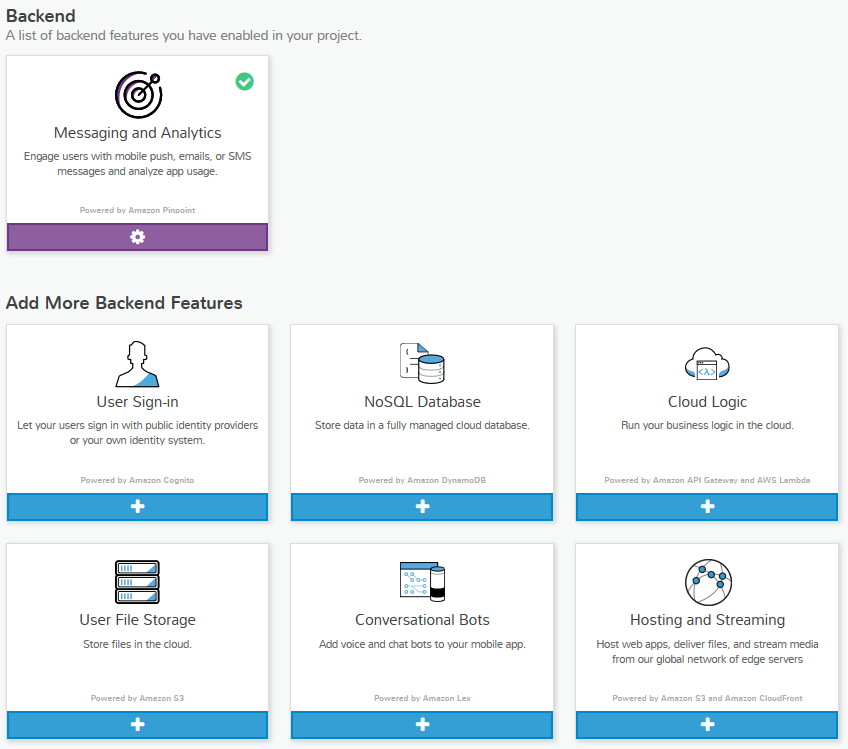
\includegraphics[width=1\linewidth]{Pictures/MobileHubBackendOverview}
	\caption[Dashboard von \gls{aws} Mobile Hub]{Dashboard von \gls{aws} Mobile Hub}
	\label{fig:mobilehubbackendoverview}
\end{figure}

\subsubsection{Login}
Ein Nutzer soll sich entweder mit E-Mail und Passwort oder Facebook authentifizieren können. 

\begin{itemize}
	\item E-Mail und Passwort:
	Dazu klicken wir in unserem Dashboard auf "User Sign-in" und wählen "E-Mail und Passwort" aus. Wir setzen das Häkchen zur Erzeugung eines neuen Benutzerverzeichnisses und legen anschließend fest, welche Anforderungen ein Passwort haben soll. Es kann festgelegt werden, wie viele und welche Zeichen das Passwort beinhalten muss. Um den Vorgang abzuschließen, klicken wir einfach "Create user pool".
	\item Facebook:
	Um Facebook als Authentifizierungsmethode zu verwenden, müssen wir zuerst uns bei der "Facebook Developer Console" anmelden und ein neues Projekt erstellen. Nach der Erzeugung des Projekts, finden wir unter "Einstellungen - Allgemeines" eine App-ID, welche wir kopieren. Nun gehen wir zurück zum \gls{aws} Mobile Hub Dashboard, klicken auf "User Sign-in" und wählen Facebook aus. Anschließend werden wir aufgefordert, die kopierte App-ID einzugeben. Ist dies erledigt, klicken wir auf "Enable Facebook Login".
\end{itemize}

Als nächstes wollen wir uns den Login in unserer Android Projekt anschauen, dazu öffnen wir die Klasse "AuthenticatorActivity" und betrachten die Methode "showSignIn()". Wir können sehen, dass sich mit nur wenigen Zeilen Code ein Login Fenster erstellen lässt, dass mit unserem Backend kommuniziert.

\subsubsection{NoSQL Datenbank}
Nun wollen wir eine Datenbank hinzufügen, in der die GPS-Daten der Kühe eines Nutzers gespeichert sind. Dazu klicken wir im Dashboard auf "NoSQL Database" und erstellen eine neue Datenbank mit dem Namen "Locations". Die Struktur der Datenbank wollen wir selbst festlegen und wählen deshalb "Costum Schema" aus. Anschließend legen wir die Datenbank Struktur wie in Abbildung \ref{fig:nosqldatabasesetup} fest und klicken anschließend "Create Table", um die Datenbank zu erstellen. Über "Download Models" kann eine Java Klasse heruntergeladen werden, die wir in unser Android Projekt einbinden. Somit können abgefragte Datensätze zu einem Java Objekt geparsed werden und wir können einfach Attribute abfragen, setzen oder ändern.

\begin{figure}[h!]
	\centering
	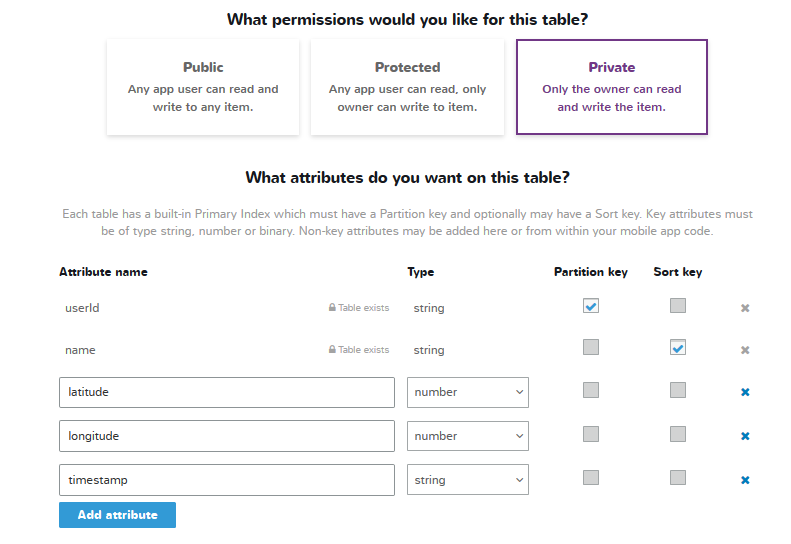
\includegraphics[width=1\linewidth]{Pictures/NoSQLDatabaseSetup}
	\caption[Datenbank Konfiguration]{Datenbank Konfiguration}
	\label{fig:nosqldatabasesetup}
\end{figure}

Schauen wir uns noch den Zugriff auf die Datenbank in der Android App an, dazu öffnen wir die Klasse "DBHandler". Durch die Methode "createLocation()" kann eine neue Position einer Kuh in der Datenbank abgespeichert werden. Mit der Methode "queryLocations()" können die Positionen aller Kühe des aktuellen Nutzers abgefragt werden. Damit wir nicht manuell neue Datensätze in die Datenbank eingeben müssen, gibt es die Methode "generateTestLocations()", die fünf Test Datensätze in die Datenbank einfügt. In der "MapsActivity" der Android App wird der "DBHandler" genutzt, um die Position der Kühe abzufragen. Diese Positionen werden dann auf einer Google Map mit einem Marker markiert. Zusätzlich wird noch via GPS der Standort des Nutzer ermittelt und ebenso mit einem Marker auf der Karte angezeigt. 

\subsubsection{Cloud Logik}
Wenn wir unsere Android App starten, haben wir bereits ein Login Fenster bei dem wir uns anmelden können und nach dem Login wird uns unsere Position und die unserer Kühe angezeigt. Nun wäre es für uns noch wichtig zu wissen, wie weit eine Kuh von uns entfernt ist. Wir gehen jetzt davon aus, dass die Berechnung der Entfernung sehr viel Ressourcen in Anspruch nimmt und wollen deshalb die Berechnung in der Cloud durchführen. Dazu klicken wir im Dashboard auf "Cloud Logic" und anschließend auf "Create a new \gls{api}". Wir füllen das Formular wie in Abbildung \ref{fig:cloudlogicsetup} aus und erstellen die \gls{api} mit "Create \gls{api}".

\begin{figure}[h!]
	\centering
	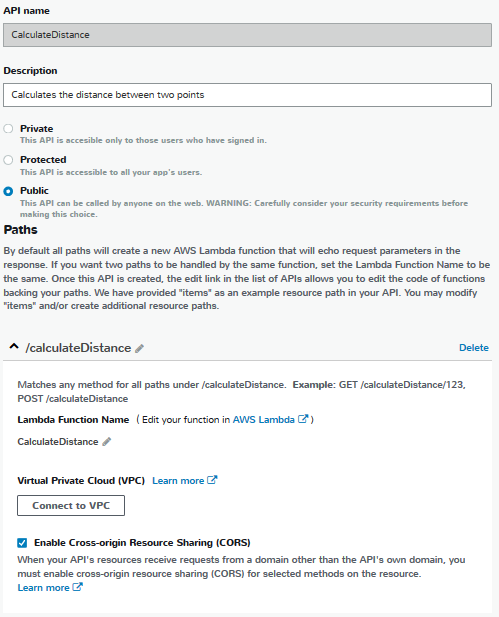
\includegraphics[width=1\linewidth]{Pictures/CloudLogicSetup}
	\caption[Cloud Logik Konfiguration]{Cloud Logik Konfiguration}
	\label{fig:cloudlogicsetup}
\end{figure}

Es wurde automatisch eine Lambda Funktion generiert, um diesen Vorgang prüfen, wählen wir den Service "Lambda Function" in unserer \gls{aws} Console aus. Wenn alles funktioniert hat, sollten wir eine Lambda Funktion mit dem Namen "CalculateDistance" sehen. Nun können wir unseren Quellcode für die Berechnung der Entfernung hinzufügen. Standardmäßig kann im Browser mit JavaScript entwickelt werden, wir bevorzugen aber Java und nutzen dafür die \gls{ide} Elipse mit dem \gls{aws} Plugin, um den Code später in die Cloud hochladen zu können. Als erstes nutzen wir das \gls{aws} Plugin um eine neues Java Lambda Projekt zu erstellen, anschließend fügen wir den Quellcode aus dem Ordner "CowTrackerLambda" unseres heruntergeladenen Git Repository ein. Nun müssen wir den Quellcode nur noch hochladen, dazu machen wir ein Rechtsklick auf das Projekt und klicken auf "Amazon Web Services - Upload function to lambda...". Es öffnet sich ein Wizard, bei dem wir die Lambda Funktion auswählen müssen, dementsprechend wählen wir "CalculateDistance" aus und klicken auf "Upload". Und schon haben wir Cloud Logik zu unserer Android App hinzugefügt. Die Cloud Logik wird in der Klasse "DistanceCalculator" der Android App über ein HTTP Anfrage abgerufen. 

\subsection{Ergebnis}
Nun haben wir alle nötigen Schritte beendet, um unsere Anforderung umzusetzen. Starten wir die App, können wir uns einloggen und die App zeigt eine Karte mit unserer Position und der Position der Kühe. Klicken wir auf einen Marker, so zeigt es uns den Kuhnamen und unsere aktuelle Entfernung zu dieser Kuh an. Abbildung \ref{fig:cowtracker} zeigt zwei Screenshots, wie das Login-Fenster und die Kartenansicht aussieht. 
\begin{figure}[!ht]
	\centering
	\begin{subfigure}{0.49\linewidth}
		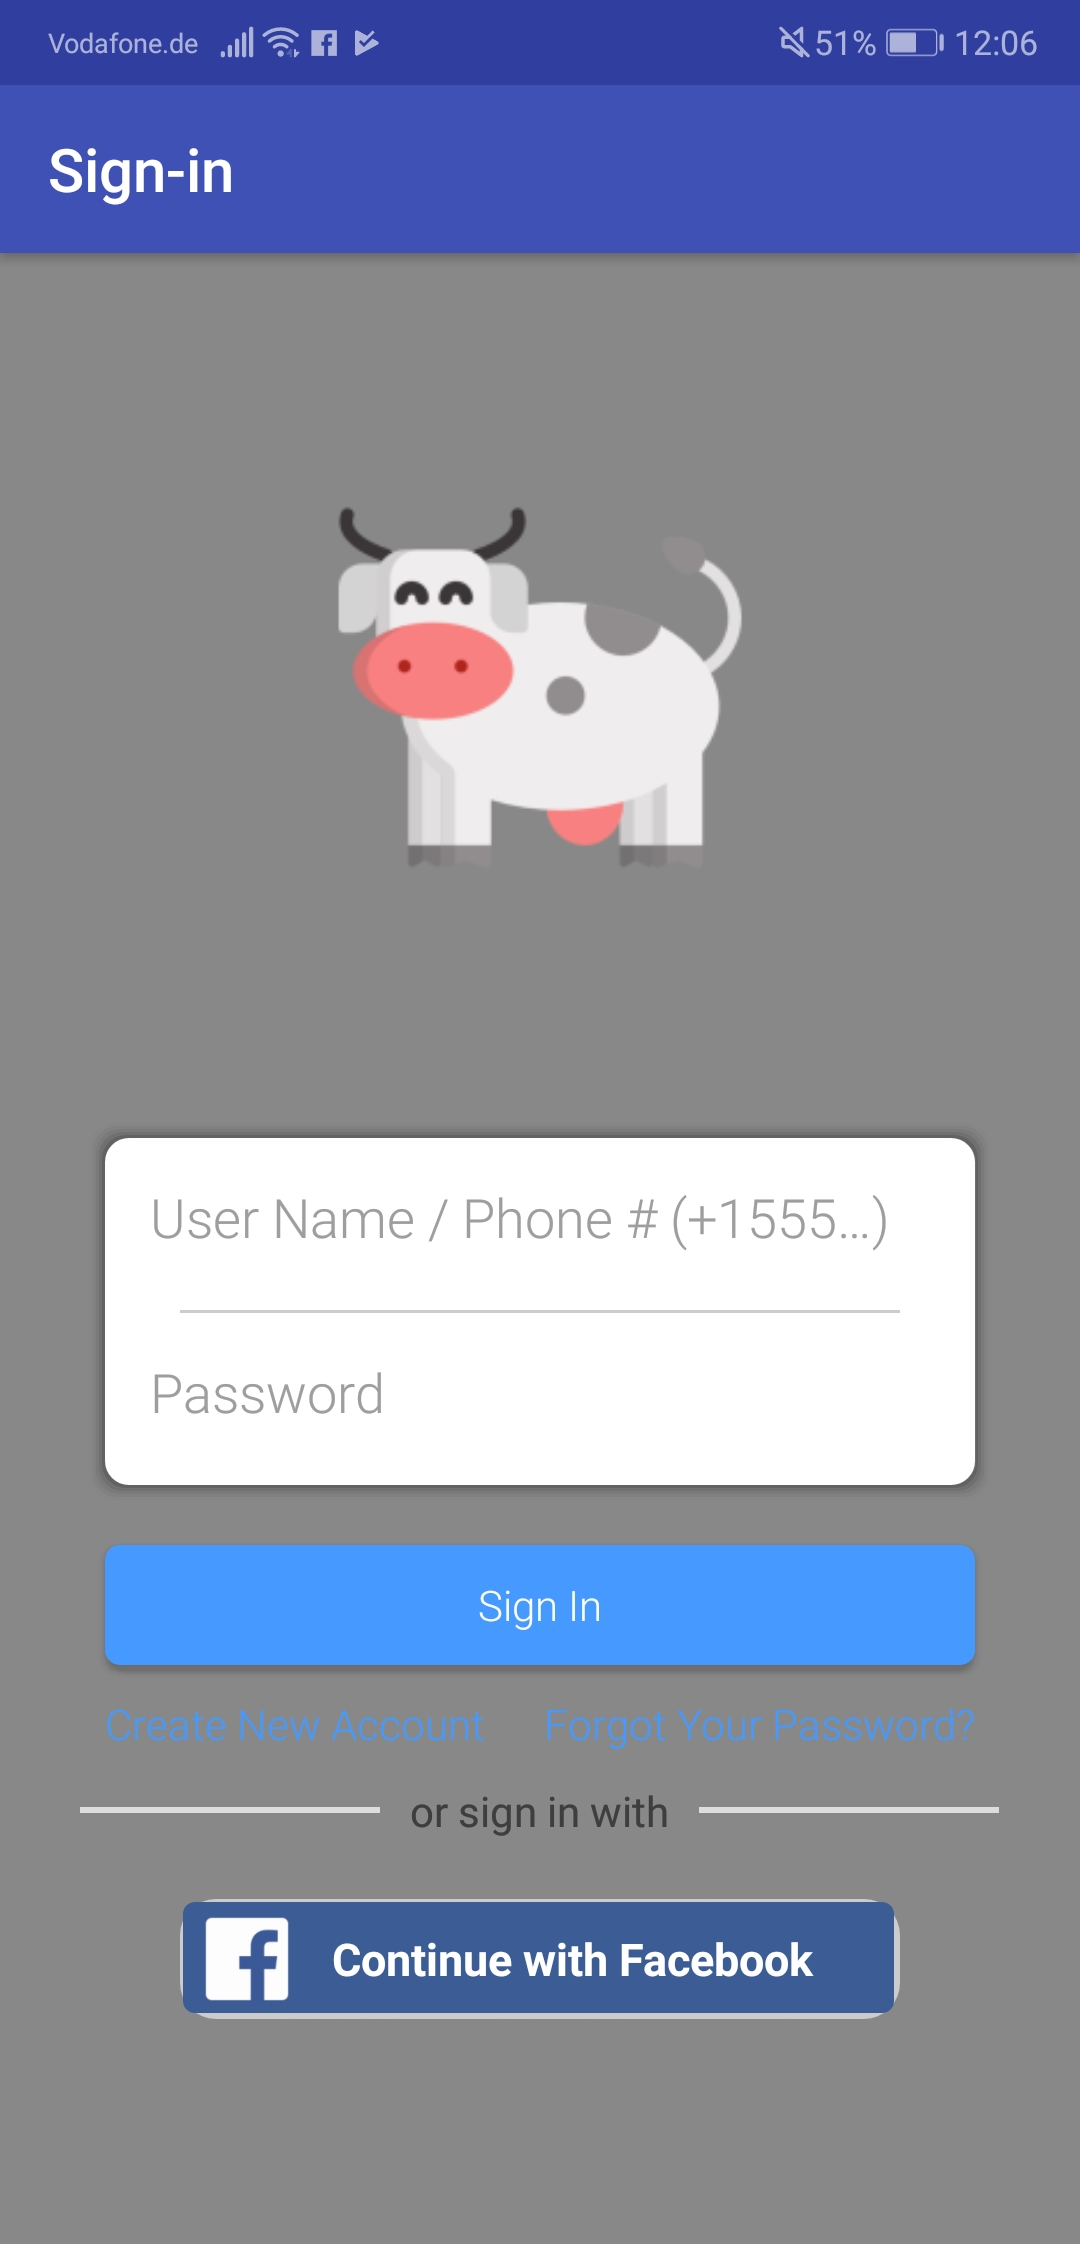
\includegraphics[width=1\linewidth]{Pictures/Screenshot_Login.jpg}
		\caption{ }
		\label{subfig:cowtracker_login}
	\end{subfigure}
	\begin{subfigure}{0.49\linewidth}
		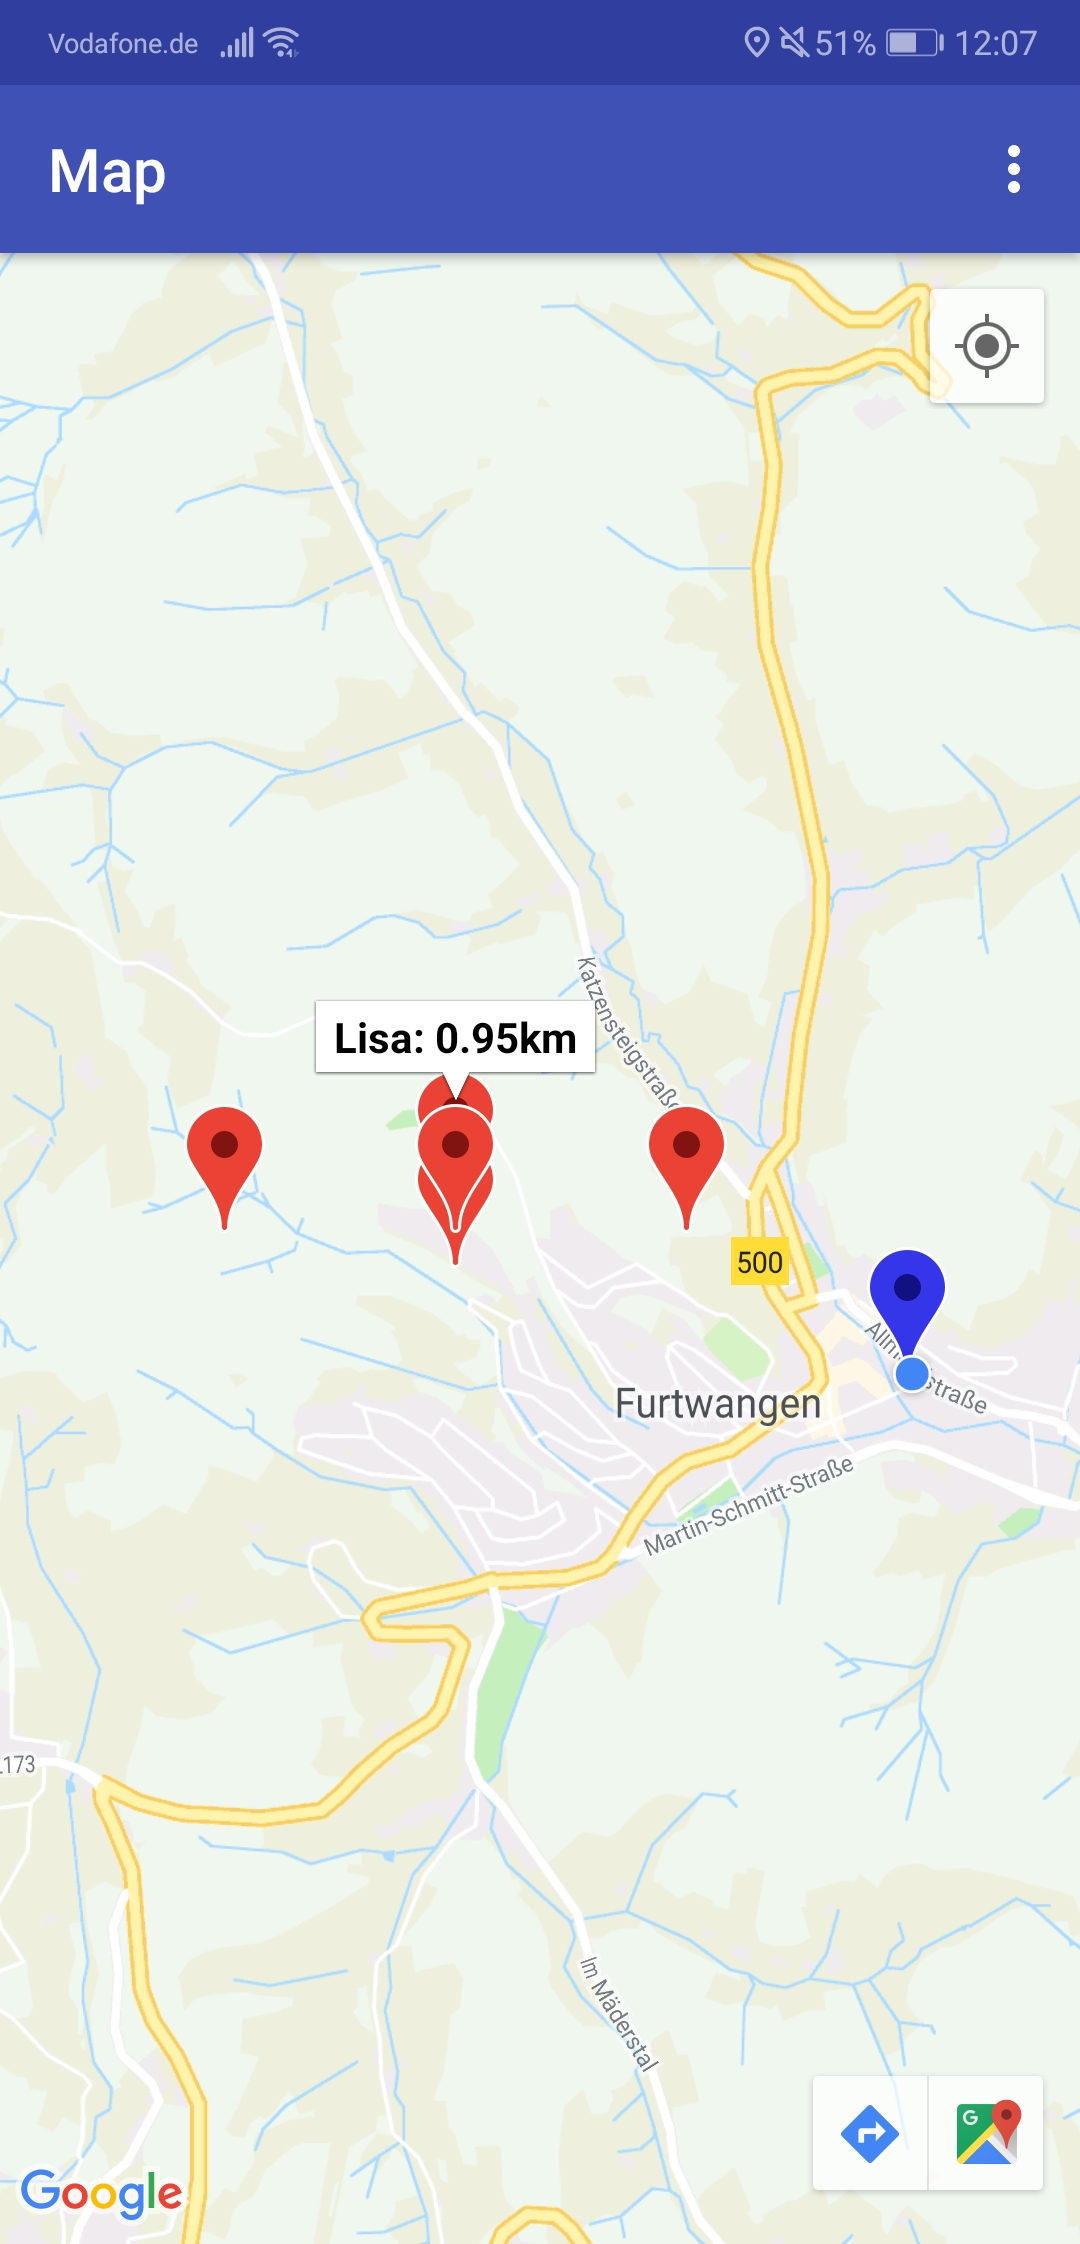
\includegraphics[width=1\linewidth]{Pictures/Screenshot_Map.jpg}
		\caption{ }
		\label{subfig:cowtracker_map}
	\end{subfigure}	
	\caption{Screenshots der Cow Tracker Android App}
	\label{fig:cowtracker}
\end{figure}

Als nächsten wollen wir noch einen kleinen Einblick in die Nutzungsstatistik werfen. Dazu wählen wir in der \gls{aws} Console den Service Pinpoint und anschließend unser Projekt aus. Nun werden uns jede Menge Statistiken zu unserer Android App angezeigt. Abbildung \ref{fig:pinpointanalystics} zeigt uns einen kleinen Ausschnitt davon. Es wird uns beispielsweise angezeigt, wie viel Nutzer die App starten oder sich pro Tag einloggen.

\begin{figure}[h!]
	\centering
	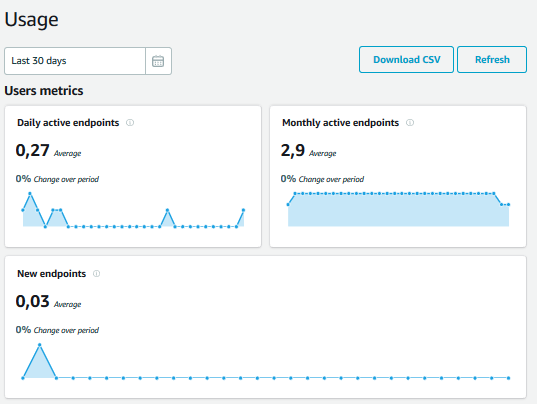
\includegraphics[width=1\linewidth]{Pictures/PinpointAnalystics}
	\caption[Pinpoint Nutzungsanalyse]{Pinpoint Nutzungsanalyse}
	\label{fig:pinpointanalystics}
\end{figure}

\section{Erfahrung}
Obwohl ich bereits mit \gls{aws} Services gearbeitet habe, habe ich mir am Anfang schwer getan mit der Konfiguration der \gls{aws} Mobile Hub. Amazon stellt eine Dokumentation und Tutorials zur Entwicklung von mobilen Anwendungen mit \gls{aws} Mobile Hub als \gls{mbaas} bereit. Jedoch unterschieden sich die verwendeten \gls{sdk} Versionen in der Dokumentationen mit der der Tutorials. Einfache Beispielanwendungen ließen sich einfach nach den Tutorials erstellen, sollten diese erweitert werden mit Funktion anhand der Dokumentation, musste genau drauf geachtet werden, welche \gls{sdk} Version genutzt wurde. Hat man mit \gls{aws} Mobile Hub eine gewisse Zeit gearbeitet und Erfahrung gesammelt, lassen sich sehr einfach Anwendungen entwickeln mit \gls{aws} als \gls{mbaas}. Ich war fasziniert, wie einfach sich \gls{aws} Cloud Services in eine Anwendungen integrieren ließen. Mit nur wenigen Zeilen Code kann eine Nutzerstatistik oder ein Login zu einer Anwendungen hinzugefügt werden. Ich werde \gls{aws} Mobile Hub in der Zukunft in den Augen behalten und falls Bedarf, für meine nächsten Anwendungen einsetzen.
\section{Fazit}
\begin{figure}[!h]
	\centering
	\includegraphics[width=0.9\linewidth]{Pictures/Fazit_Grafik}
	\caption[Verbesserung der MMI durch Emotion Tracking]{Verbesserung der MMI durch Emotion Tracking}
	\label{fig:fazitgrafik}
\end{figure}


% *** END OF SECTIONS ***---------------------------------------------

% needed in second column of first page if using \IEEEpubid
%\IEEEpubidadjcol

% An example of a floating figure using the graphicx package.
% Note that \label must occur AFTER (or within) \caption.
% For figures, \caption should occur after the \includegraphics.
% Note that IEEEtran v1.7 and later has special internal code that
% is designed to preserve the operation of \label within \caption
% even when the captionsoff option is in effect. However, because
% of issues like this, it may be the safest practice to put all your
% \label just after \caption rather than within \caption{}.
%
% Reminder: the "draftcls" or "draftclsnofoot", not "draft", class
% option should be used if it is desired that the figures are to be
% displayed while in draft mode.
%
%\begin{figure}[!t]
%\centering
%\includegraphics[width=2.5in]{myfigure}
% where an .eps filename suffix will be assumed under latex, 
% and a .pdf suffix will be assumed for pdflatex; or what has been declared
% via \DeclareGraphicsExtensions.
%\caption{Simulation Results}
%\label{fig_sim}
%\end{figure}

% Note that IEEE typically puts floats only at the top, even when this
% results in a large percentage of a column being occupied by floats.


% An example of a double column floating figure using two subfigures.
% (The subfig.sty package must be loaded for this to work.)
% The subfigure \label commands are set within each subfloat command, the
% \label for the overall figure must come after \caption.
% \hfil must be used as a separator to get equal spacing.
% The subfigure.sty package works much the same way, except \subfigure is
% used instead of \subfloat.
%
%\begin{figure*}[!t]
%\centerline{\subfloat[Case I]\includegraphics[width=2.5in]{subfigcase1}%
%\label{fig_first_case}}
%\hfil
%\subfloat[Case II]{\includegraphics[width=2.5in]{subfigcase2}%
%\label{fig_second_case}}}
%\caption{Simulation results}
%\label{fig_sim}
%\end{figure*}
%
% Note that often IEEE papers with subfigures do not employ subfigure
% captions (using the optional argument to \subfloat), but instead will
% reference/describe all of them (a), (b), etc., within the main caption.


% An example of a floating table. Note that, for IEEE style tables, the 
% \caption command should come BEFORE the table. Table text will default to
% \footnotesize as IEEE normally uses this smaller font for tables.
% The \label must come after \caption as always.
%
%\begin{table}[!t]
%% increase table row spacing, adjust to taste
%\renewcommand{\arraystretch}{1.3}
% if using array.sty, it might be a good idea to tweak the value of
% \extrarowheight as needed to properly center the text within the cells
%\caption{An Example of a Table}
%\label{table_example}
%\centering
%% Some packages, such as MDW tools, offer better commands for making tables
%% than the plain LaTeX2e tabular which is used here.
%\begin{tabular}{|c||c|}
%\hline
%One & Two\\
%\hline
%Three & Four\\
%\hline
%\end{tabular}
%\end{table}


% Note that IEEE does not put floats in the very first column - or typically
% anywhere on the first page for that matter. Also, in-text middle ("here")
% positioning is not used. Most IEEE journals use top floats exclusively.
% Note that, LaTeX2e, unlike IEEE journals, places footnotes above bottom
% floats. This can be corrected via the \fnbelowfloat command of the
% stfloats package.









% if have a single appendix:
%\appendix[Proof of the Zonklar Equations]
% or
%\appendix  % for no appendix heading
% do not use \section anymore after \appendix, only \section*
% is possibly needed

% use appendices with more than one appendix
% then use \section to start each appendix
% you must declare a \section before using any
% \subsection or using \label (\appendices by itself
% starts a section numbered zero.)
%


% use section* for acknowledgement
%\section*{Acknowledgment}


%The authors would like to thank...


% Can use something like this to put references on a page
% by themselves when using endfloat and the captionsoff option.
\ifCLASSOPTIONcaptionsoff
  \newpage
\fi



% trigger a \newpage just before the given reference
% number - used to balance the columns on the last page
% adjust value as needed - may need to be readjusted if
% the document is modified later
%\IEEEtriggeratref{8}
% The "triggered" command can be changed if desired:
%\IEEEtriggercmd{\enlargethispage{-5in}}

% references section

% can use a bibliography generated by BibTeX as a .bbl file
% BibTeX documentation can be easily obtained at:
% http://www.ctan.org/tex-archive/biblio/bibtex/contrib/doc/
% The IEEEtran BibTeX style support page is at:
% http://www.michaelshell.org/tex/ieeetran/bibtex/
%\bibliographystyle{IEEEtran}
% argument is your BibTeX string definitions and bibliography database(s)
%\bibliography{IEEEabrv,../bib/paper}
%
% <OR> manually copy in the resultant .bbl file
% set second argument of \begin to the number of references
% (used to reserve space for the reference number labels box)
\begin{thebibliography}{1}
\bibitem{AmazonLambda}
"Amazon Lambda"
\url{https://aws.amazon.com/de/lambda/} 
Accessed 18.06.2018

\bibitem{AmazonDynamoDB}
"Amazon DynamoDB"
\url{https://aws.amazon.com/de/dynamodb/}
Accessed 18.06.2018

\bibitem{AmazonCloudWatch}
"Amazon Cloud Watch"
\url{https://aws.amazon.com/de/cloudwatch/}
Accessed 18.06.2018

\bibitem{AmazonPinpoint}
"Amazon Pinpoint"
\url{https://aws.amazon.com/de/pinpoint/}
Accessed 18.06.2018

\bibitem{AmazonCognito}
"Amazon Cognito"
\url{https://aws.amazon.com/de/cognito/}
Accessed 19.06.2018

\bibitem{AmazonAPIGateway}
"Amazon \gls{api} Gateway"
\url{https://aws.amazon.com/de/api-gateway/}
Accessed 20.06.2018

\bibitem{AmazonE3}
"Amazon E3"
\url{https://aws.amazon.com/de/s3}
Accessed 20.06.2018

\bibitem{AmazonLex}
"Amazon Lex"
\url{https://aws.amazon.com/de/lex}
Accessed 20.06.2018

\bibitem{AmazonCloudFront}
"Amazon Cloud Front"
\url{https://aws.amazon.com/de/cloudfront/}
Accessed 20.06.2018

\bibitem{techbeacon}
"TechBeacon - How choose right MBaas"
\url{https://techbeacon.com/how-choose-right-mbaas-google-firebase-apple-icloud-or-kinvey}
Accessed 18.06.2018

\bibitem{applecloudkit}
"Apple Cloud Kit"
\url{https://developer.apple.com/documentation/cloudkit}
Accessed 18.06.2018

\bibitem{progresskinvey}
"Progress Kinvey"
\url{https://www.progress.com/kinvey/}
Accessed 18.06.2018

\bibitem{googlefirebase}
"Google Firebase"
\url{https://firebase.google.com/}
Accessed 18.06.2018

\bibitem{kumulos}
"Kumulos"
\url{https://www.kumulos.com/}
Accessed 19.06.2018

\bibitem{canival}
"Karnival - 5 best \gls{mbaas} alternatives to parse"
\url{http://carnival.io/mobile-insights/5-best-mbaas-alternatives-to-parse-2/}
Accessed 19.06.2018

\bibitem{back4app}
"back4app"
\url{https://www.back4app.com/}
Accessed 19.06.2018

\bibitem{parse}
"Parse"
\url{https://www.back4app.com/}
Accessed 19.06.2018

\bibitem{statistacloudmarketshare}
"Statista - Cloud Market Share"
\url{https://www.statista.com/chart/7994/cloud-market-share/}

\end{thebibliography}

% biography section
% 
% If you have an EPS/PDF photo (graphicx package needed) extra braces are
% needed around the contents of the optional argument to biography to prevent
% the LaTeX parser from getting confused when it sees the complicated
% \includegraphics command within an optional argument. (You could create
% your own custom macro containing the \includegraphics command to make things
% simpler here.)
%\begin{biography}[{\includegraphics[width=1in,height=1.25in,clip,keepaspectratio]{mshell}}]{Michael Shell}

% You can push biographies down or up by placing
% a \vfill before or after them. The appropriate
% use of \vfill depends on what kind of text is
% on the last page and whether or not the columns
% are being equalized.

%\vfill

% Can be used to pull up biographies so that the bottom of the last one
% is flush with the other column.
%\enlargethispage{-5in}



% that's all folks
\end{document}


